\documentclass[10pt,a4paper]{beamer}
\usepackage[utf8]{inputenc}
\usepackage[german]{babel}
\usepackage{amsmath}
\usepackage{amsfonts}
\usepackage{amssymb}
\usepackage{graphicx}
\usepackage{lmodern}
\usepackage{color}
\usepackage{listings} 
\usepackage{algorithm2e}
\usepackage{tabularx} 
\usepackage{xcolor,colortbl}
\usepackage{arydshln}

\lstset{numbers=left, numberstyle=\tiny, numbersep=5pt} 
\lstset{language=html}

\author{Mirko Hering, Julia Kreutzer, Jasmin Schröck}
\title{Sentiment Classification}
\subtitle{Multi-Task-Learning und l1/l2-Regularisierung}
%\titlegraphic{\includegraphics[scale=•]{•}=4cm,height=3cm]{MediaWiki-notext.pdf}}

\definecolor{unihdred}{RGB}{153, 0, 0}
\definecolor{yellow}{RGB}{255, 255, 0}
\definecolor{rosa}{RGB}{244, 204, 204}

\usecolortheme[RGB={153, 0, 0}]{structure}
\usepackage{beamerthemesplit}

\begin{document}

\frame{
	\titlepage
}

\frame{
	\frametitle{Inhaltsverzeichnis}
	\tableofcontents[hideallsubsections]
}

\section{Aufgabenstellung und Lösungsansatz}
\frame{
	\begin{center}
	\huge{Aufgabenstellung und Lösungsansatz}\\
	\LARGE{- Spezifikation revived}
	\end{center}
}

\subsection{Aufgabenstellung}
\frame{
	\frametitle{Aufgabenstellung}
	\large{Ziel}
	\begin{itemize}
	\item Gewinnung von Features, die für alle Kategorien der Testdaten aussagekräftig und bei der Klassifizierung nützlich sind
	\item Lernverfahren auf bewertete Produktrezensionen von Amazon.com anwenden, mit Hilfe der gewonnenen Features in positiv und negativ klassifizieren
	\end{itemize}
}

\subsection{Lösungsansatz}
\frame{
	\frametitle{Lösungsansatz}
	\begin{itemize}
	\item Anwendung von Multitask-Learning mit verteilter l1/l2- Regularisierung zur Feature-Selektion
	\item Die Produktkategorien (books, dvd, electronics, kitchen) entsprechen den Tasks des Multi-Task-Learnings
	\item Alternativ zu Produktkategorien: Random Shards
	\end{itemize}
}

\section{Umsetzung}
\frame{
	\begin{center}
	\huge{Umsetzung}\\
	\LARGE{- Implementierung, Hadoop und Co.}
	\end{center}
}
\subsection{Daten}
\frame{
	\frametitle{Daten}
	\large{Multi-Domain Sentiment Dataset (version 2.0)}
	\begin{itemize}
	\item Englischsprachige Produktrezensionen von Amazon.com
	\item 4 Kategorien: Bücher, DVDs, Küchengeräte, Elektronik
	\item Rezensionen sind positiv und negativ gelabelt
	\item Preprocessed: Zählung von Unigrammen und Bigrammen
	\item für jede Kategorie 1000 negative und 1000 positive Rezensionen
	\end{itemize}
}
\frame{
	\frametitle{Daten}
	\large{Unsere Aufteilung:}
	\begin{itemize}
	\item je 1200 Rezensionen für Training 
	\item und je 400 für Test und Development
	\end{itemize}
}

\subsection{Methoden}
\frame{
	\frametitle{Methoden}
	\large{Parameter:}
	\begin{itemize}
	\item Lernrate $\eta^{t}$
	\item Epochenzahl t\\
	\begin{small}
	-diese wird durch die Laufzeit auf Hadoop begrenzt werden
	\end{small}
	\item Gewichtsvektorinitialisierung $v_{0}$
	\item Auswahl der top k Features
	\item Anzahl/Daten in shards Z\\
	\begin{small}
	-4 Kategorien, also 4 Shards
	\end{small}
	\end{itemize}
}

\subsection{Korpusformat}
\frame{
	\frametitle{Korpusformat}
	\begin{itemize}
	\item Format einer Rezension:\\
	{\small Kategorie	feature:count feature:count (...) \#label\#:[positive$\vert$negative]}
	\item Format des Korpus: eine Rezension pro Zeile\\[0.5cm]
	\end{itemize}
	
	{\large 6 Korpora:}
	\begin{itemize}
	\item Je ein Korpus mit allen Rezensionen einer Kategorie
	\item Plus ein Korpus mit allen Rezensionen (pooled - all)
	\item Plus ein Korpus mit Rezensionen aus allen Kategorien, jedoch nur so groß wie ein Korpus einer einzelnen Kategorie (pooled - small)

	\end{itemize}
}

\subsection{Klassenarchitektur}
\frame{
	\frametitle{Klassenarchitektur}
	\Huge{To do!}
}
\frame{
	\frametitle{Klassenarchitektur}
	\Huge{To do!}
}

\subsection{Hadoop}
\frame{
	\frametitle{Hadoop - MT Learning}
	\begin{itemize}
	\item Aufruf der jar-Datei mit Hadoop
	\item Angabe der Parameter (top k Features, Epochen, Kategorien) \\[0.5cm]
	\item Innerhalb einer Epoche: Durchlauf der Phasen 1 \& 2
	\item Abschließend: Selektion der top k Features
	\end{itemize}
}
\frame{
	\frametitle{Hadoop - MT Learning}
	\begin{center}
	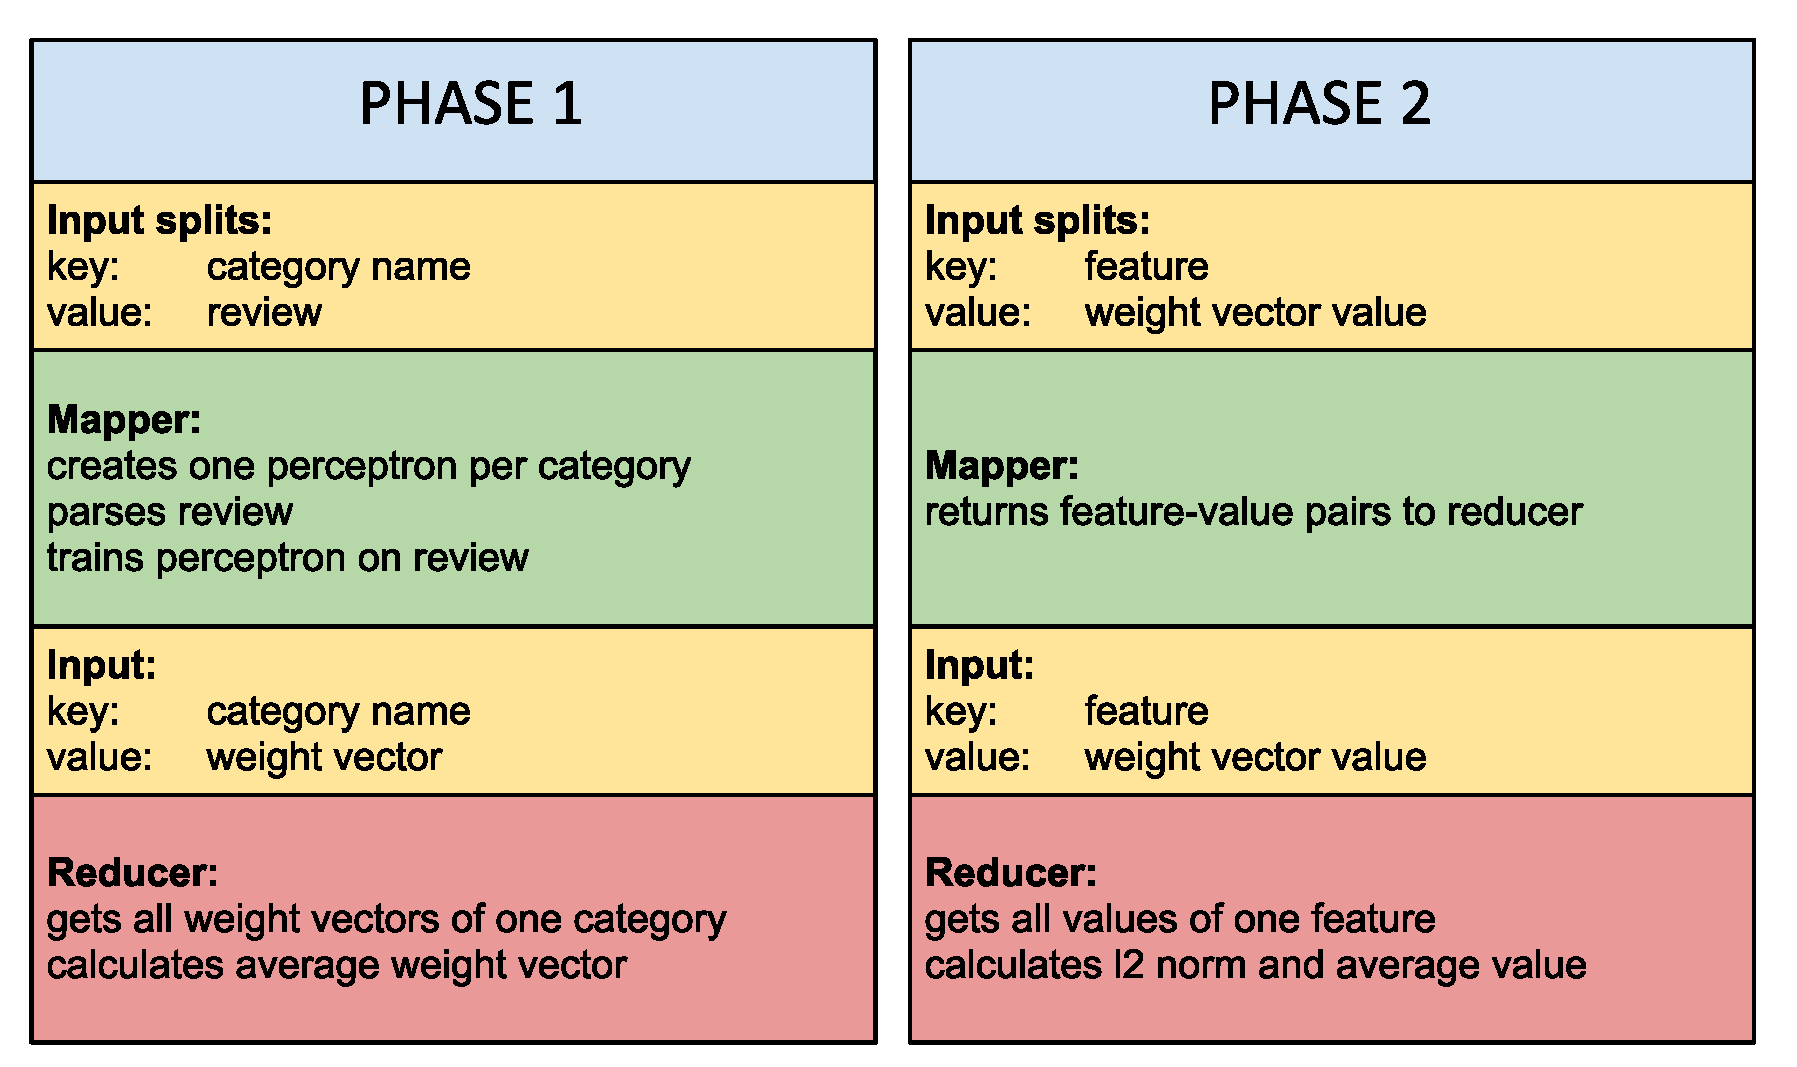
\includegraphics[scale=0.35]{MapReducePhases.pdf} 
	\end{center}

}
\frame{
	\frametitle{Hadoop - Random Shards}
	\begin{center}
	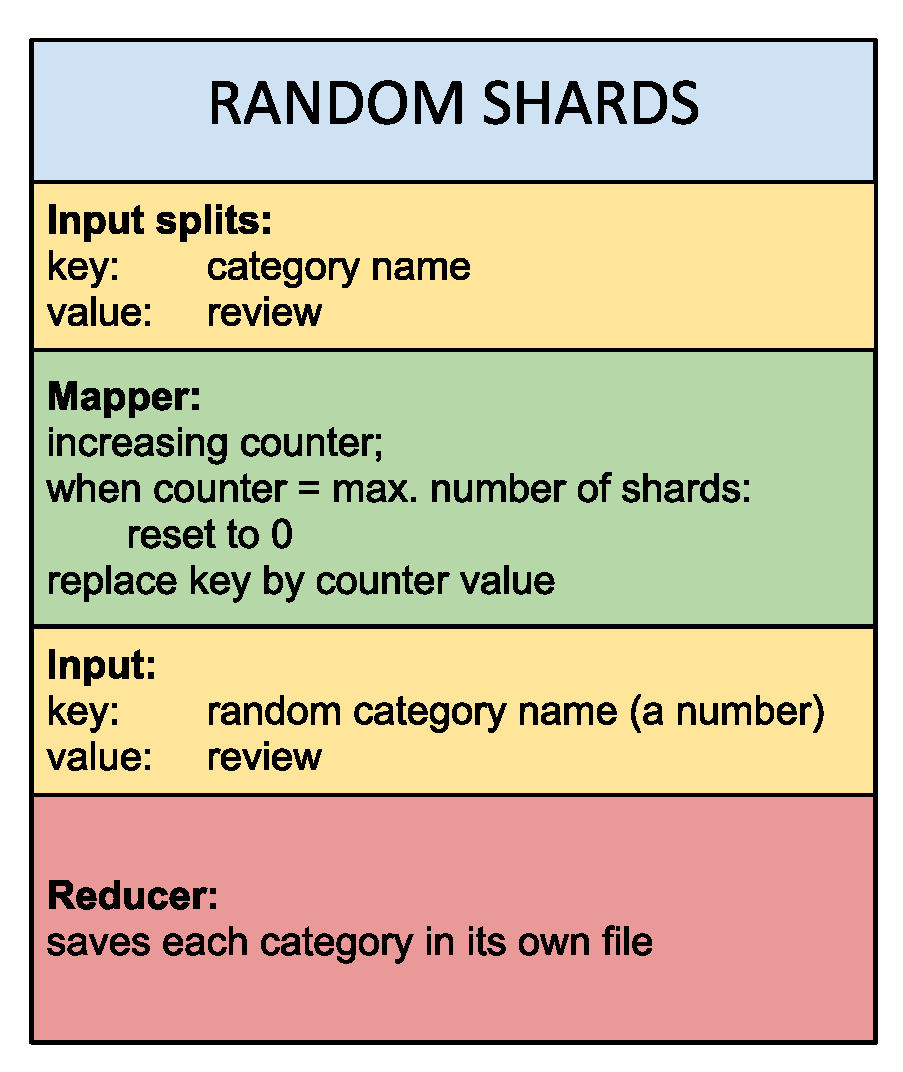
\includegraphics[scale=0.35]{RandomShards.pdf} 
	\end{center}

}
\frame{
	\frametitle{Parameter-Optimierung}
	{\large Maß: Error-Rate}
	\begin{itemize}
	\item Lernrate $\eta^{t}$: $10, 10^{-1}, 10^{-2}, 10^{-3}, 10^{-4}, 10^{-5}, 10^{-6}, \dfrac{1}{t}, exp, dec$\\

	exp: {\scriptsize $1*0,85^{^{\dfrac{-t}{trainsetSize}}}$}\\[0.5cm]
	dec: {\scriptsize $\dfrac{1}{1+\dfrac{t}{trainsetSize}}$}		

	\item Epochenzahl t: 1, 10, 20, 30
	\item Gewichtsvektorinitialisierung $v_{0}=0$
	\item Auswahl der top k Features:\\
	$k=10, 100, 1.000, 2.000, 5.000, 10.000, 50.000$
	\item Anzahl der shards Z: 4
	\end{itemize}
}

\frame{
	\frametitle{Parameter-Optimierung}
	{\large weitere Experimente:}
	\begin{itemize}
	\item Margin Perceptron (update if $y_{i} \langle x_{i},w_{z},t \rangle <= 1$)
	\item Word Net (Synsets für Unigramme)\\[1cm]
	\item Jedoch keine Verbesserung :-(
	\end{itemize}
}

\frame{
	\frametitle{Hadoop - Random Shards}
	\begin{center}
	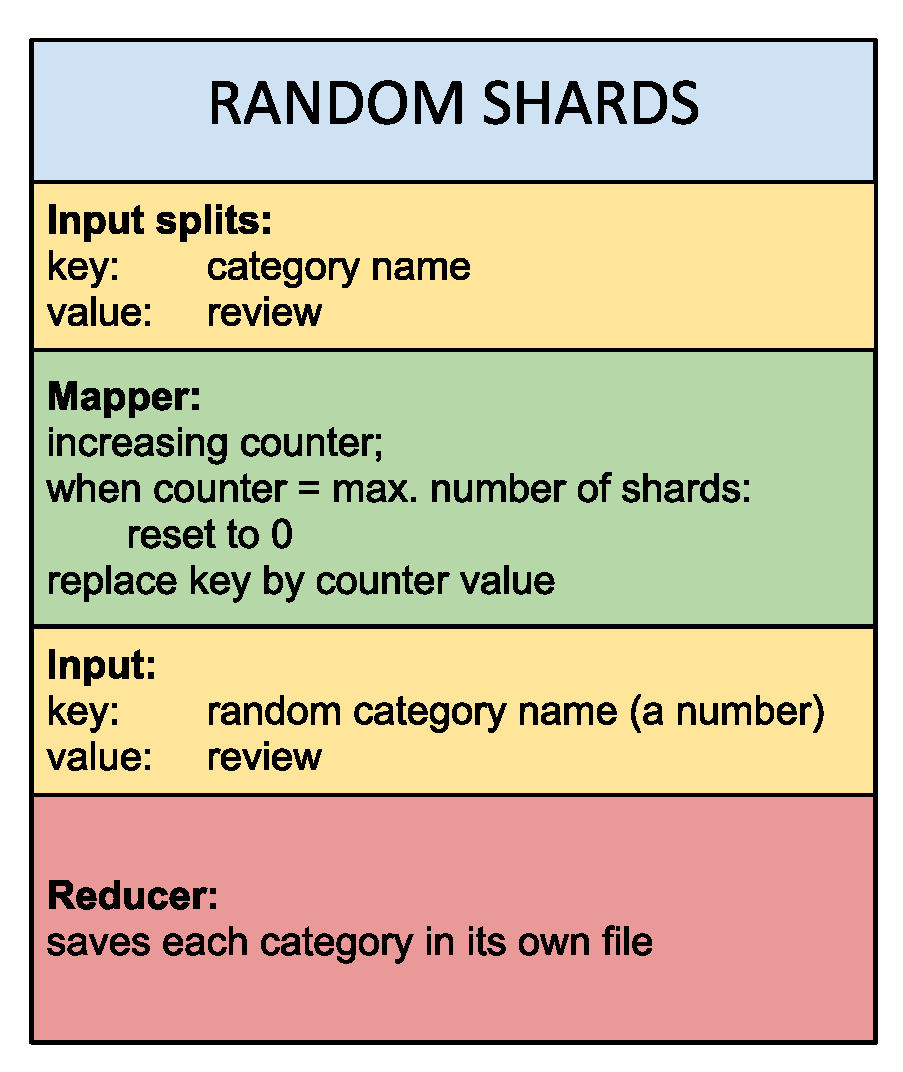
\includegraphics[scale=0.35]{RandomShards.pdf} 
	\end{center}

}
\frame{
	\frametitle{Parameter-Optimierung}
	{\large Maß: Error-Rate}
	\begin{itemize}
	\item Lernrate $\eta^{t}$: $10, 10^{-1}, \textcolor{red}{10^{-2}}, 10^{-3}, 10^{-4}, 10^{-5}, 10^{-6}, \dfrac{1}{t}, exp, dec$\\

	\item Epochenzahl t: 1, \textcolor{red}{10}, 20, 30
	\item Auswahl der top k Features:\\
	$k=10, 100, 1.000, 2.000, \textcolor{red}{5.000}, 10.000, 50.000$\\[1cm]
	\end{itemize}
	{\large Optimale Parameter:}\\
	10 Epochen, Lernrate = $10^{-2}$, top 5000 Features
}

\section{Evaluation}
\frame{
	\begin{center}
	\huge{Evaluationsergebnisse}\\
	\LARGE{- sprechende Zahlen}
	\end{center}
}

\subsection{Baselines}
\frame{
	\frametitle{Wie gut klassifiziert unser regularisierter Multi-Task Perceptron...}
	\begin{itemize}
	\item ... jede einzelne Kategorie?
	\item ... im Vergleich zu Single-Task Learning?
	\item ... im Vergleich zu random sharded Multi-Task Learning? \\[1cm]
	\end{itemize}
	{\large Baselines:}
	\begin{itemize}
	\item Single-Task-Learning auf einzelnen Kategorien
	\item Single-Task-Learning auf allen Daten
	\item Multi-Task-Learning mit random shards
	\end{itemize}
}

\subsection{Fakten, Fakten, Fakten}
\frame{
	\frametitle{Single Task Learning}
	\newcolumntype{Y}{>{\columncolor{yellow}}c}
	\begin{center}
		\resizebox{10cm}{!} {
			\begin{tabular}{ l | c c Y }
					&	\textbf{independent}	&	\textbf{small}	&	\textbf{all}		\\ \hline
		books		&	0,2275		&	0,3000	&	0,1925\\
		dvd			&	0,2200		&	0,2750	&	0,2000	\\
		electronics	&	0,1825		&	0,2100	&	0,1525	\\
		kitchen		&	0,1475		&	0,2325	&	0,1425	\\ \hline
		average		&	0,1944		&	0,2544	&	0,1719	
			\end{tabular}
		},
	\end{center}
}

\frame{
	\frametitle{Multi Task Learning}
	\begin{center}
		\resizebox{10cm}{!} {
			\begin{tabular}{ l | c c }
					&	\textbf{shards = tasks}	&	\textbf{random shards}	\\ \hline
		books		&	\cellcolor{yellow}0,2375		&	0,2400	\\
		dvd			&	0,2175		&	\cellcolor{yellow}0,1900	\\
		electronics	&	0,1550		&	\cellcolor{yellow}0,1500	\\
		kitchen		&	\cellcolor{yellow}0.1450		&	0,1525	\\ \hline
		average		&	0,1888		&	\cellcolor{yellow}0,1831
			\end{tabular}
		}
	\end{center}
}
\frame{
	\frametitle{Vergleich}
	\begin{center}
		\resizebox{10cm}{!} {
			\begin{tabular}{ l | c | c }
					&	\textbf{average error rate}	&	\textbf{average vector length}	\\ \hline
		ST independent		&	0,1944		&	63.213	\\
		ST small			&	0,2544		&	78.089	\\
		\rowcolor{rosa} 
		ST all				&	0,1719		&	194.627	\\ \hdashline
		\rowcolor{yellow} 
		MT shards = tasks	&	0,1888		&	5.000	\\
		\rowcolor{yellow}
		MT random shards	&	0,1831		&	5.000
			\end{tabular}
		}
	\end{center}
}

\subsection{Unseen Corpora}
\frame{
	\frametitle{Unseen Corpora}
	Erstellung zusätzlicher Testcorpora:
	\begin{itemize}
	\item Herunterladen von Amazon-Kundenrezensionen:\\
	http://www.esuli.it/fossil/repo/amazonReviewsDownloader/index
	\item eigenes Python-Skript zum Formatieren \\[0.5cm]
	\end{itemize}
	Korpora haben unterschiedliche Längen und sind nicht ausgeglichen:
\begin{scriptsize}
	\begin{center}
		\resizebox{8cm}{!} {
			\begin{tabular}{ c c c }
			Kategorie	&	Rezensionen	&	Anteil positiv\\ \hline
			gardening	&	1865		&	0,8\\
			outdoor		&	916			&	0,86\\
			snacks		&	208			&	0,95\\
			organicfood	&	97211		&	0,88\\
			\end{tabular}
		}
	\end{center}
\end{scriptsize}
}

\frame{
	\frametitle{Unseen Corpora}
	\begin{center}
%		\resizebox{6cm}{!} {
			\begin{tabular}{ c | c }
					&	\parbox{5cm}{\centering\textbf{average error rate \\ on unseen test corpora}}	\\ \hline
			ST independent	&	0,2611 \\
				books		&	0,4164 \\
				dvd			&	0,2997 \\
				electornics	&	0,1873 \\
	    	\rowcolor{yellow}
				kitchen		&	0,1410 \\
			ST small		&	0,2253 \\
			ST all			&	0,1781 \\\hdashline
			\rowcolor{yellow}
			MT shards = tasks &	0,1616 \\
			MT random shards &	0,1776 \\
			\end{tabular}
%		}
	\end{center}
}

\subsection{Unseen Corpora}
\frame{
	\frametitle{Unseen Corpora}
	Erstellung zusätzlicher Testcorpora:
	\begin{itemize}
	\item Herunterladen von Amazon-Kundenrezensionen:\\
	http://www.esuli.it/fossil/repo/amazonReviewsDownloader/index
	\item eigenes Python-Skript zum Formatieren \\[0.5cm]
	\end{itemize}
	Korpora haben unterschiedliche Längen und sind nicht ausgeglichen:
\begin{scriptsize}
	\begin{center}
		\resizebox{8cm}{!} {
			\begin{tabular}{ c c c }
			Kategorie	&	Rezensionen	&	Anteil positiv\\ \hline
			gardening	&	1865		&	0,8\\
			outdoor		&	916			&	0,86\\
			snacks		&	208			&	0,95\\
			organicfood	&	97211		&	0,88\\
			\end{tabular}
		}
	\end{center}
\end{scriptsize}
}


\section{Demo}
\frame{
	\huge{}
}
\frame{
	\frametitle{}

}
\section{Fazit}
\frame{
	\huge{}
}
\frame{
	\frametitle{}

}
\section{Referenzen}
\frame{
	\huge{}
}
\frame{
	\frametitle{}

}

\end{document}